\documentclass[a4paper]{report}
\usepackage{a4wide}
\usepackage[utf8]{inputenc}
\usepackage[T1]{fontenc}
\usepackage{parskip}
\usepackage{hyperref}
\usepackage{epsfig}
\usepackage{background}
\usepackage{mathptmx}

% To avoid tikz error, see https://tex.stackexchange.com/questions/165929/semiverbatim-with-tikz-in-beamer
\makeatletter
\global\let\tikz@ensure@dollar@catcode=\relax
\makeatother

\backgroundsetup{
scale=1,
angle=0,
opacity=1,
contents={
\includegraphics[width=\paperwidth,height=\paperheight]{images/spi-front.jpg}}
}

\hypersetup{
  colorlinks   = true,
  urlcolor     = blue,
  linkcolor    = blue,
  pdfinfo = {
    Title = {SPI Annual Report 2024},
    Author = {Software in the Public Interest, Inc.},
    Keywords = {SPI, free software, open source, FOSS, annual report, charity, non-profit, 501c3},
  }
}

\begin{document}

\title{Software in the Public Interest, Inc.\\
2024 Annual Report}
\date{July XXX, 2025}

\maketitle

\newpage

\backgroundsetup{
scale=1,
angle=0,
opacity=1,
contents={
\includegraphics[width=\paperwidth,height=\paperheight]{images/spi-content.jpg}}
}

\hspace{1em}

To the membership, board and friends of Software in the Public Interest, Inc:

As mandated by Article 8 of the SPI Bylaws, I respectfully submit this annual report on the activities of Software in the Public Interest, Inc. and extend my thanks to all of those who contributed to the mission of SPI in the past year.

  \emph{-- Michael Schultheiss, SPI President}

\newpage

\tableofcontents

\newpage

\chapter{Committee Reports}
\section{Membership Committee}

\subsection{Statistics}

On January 1, 2024 we had 198 contributing and 1422 non-contributing members.  On December 31, 2024 there were XXX contributing members and XXX non-contributing members.

\chapter{Board Report}
\section{Board Members}

Board members as of January 1, 2024:

\begin{itemize}
\item Michael Schultheiss (President)
\item Stephen Frost (Vice President)
\item Zach van Rijn (Secretary)
\item Héctor Orón Martínez (Treasurer)
\item Joe Conway
\item Forrest Fleming
\item Milan Kupcevic
\item Jonatas L. Nogueira
\item Jeremy Stanley
\end{itemize}

Board members as of December 31, 2024:

\begin{itemize}
\item Michael Schultheiss (President)
\item Jonatas L. Nogueira (Vice President)
\item Zach van Rijn (Secretary)
\item Héctor Orón Martínez (Treasurer)
\item Joe Conway
\item Forrest Fleming
\item Milan Kupcevic
\item Katherine McMillan
\item Jeremy Stanley
\end{itemize}

\section{Board Changes}

Changes that occurred during the year:

\begin{itemize}

\item The terms for Stephen Frost, Milan Kupcevic, and Michael Schultheiss expired in July 2024.  Milan Kupcevic and Michael Schultheiss sought, and obtained, re-election.  We'd like to thank Stephen Frost for his work on the board.  Katherine (Katie) McMillan joined the board as part of the same election.

\item On August 12, 2024 the board voted to appoint the following officers:

\begin{itemize}
\item President: Michael Schultheiss
\item Vice President: Jonatas L. Nogueira
\item Secretary: Zach van Rijn
\item Treasurer: Héctor Orón Martínez
\end{itemize}

\end{itemize}

\section{Elections}

A board membership election was conducted in July 2024.  There were 3 board seats up for election.  Nominations were received from Milan Kupcevic, Katherine (Katie) McMillan, and Michael Schultheiss.  Since there was 3 nominations for 3 board seats, no vote was required and the candidates were elected for a 3 year term.

\chapter{Treasurer's Report}

SPI will publish audited financial statements soon (approximately August 2025).

\chapter{Member Project Reports}

\section{New Associated Projects}

\subsection{Gentoo Linux}

\href{https://www.gentoo.org/}{Gentoo Linux} is a free operating system based on Linux that can be automatically optimized and customized for just about any application or need. Extreme configurability, performance, and a top-notch user and developer community are all hallmarks of the Gentoo experience.

\subsection{Rocket}

\href{https://rocket.rs/}{Rocket} is a web framework for Rust that makes it simple to write fast, type-safe, secure web applications with incredible usability, productivity and performance.

\section{Updates from Associated Projects}

\appendix
\chapter{About SPI}

SPI is a non-profit organization which was founded to help organizations develop and distribute open hardware and software. We encourage programmers to use the GNU General Public License or other licenses that allow free redistribution and use of software, and hardware developers to distribute documentation that will allow device drivers to be written for their product.

SPI was incorporated as a non-profit organization on June 16, 1997 in the state of New York. Since then, it has become an umbrella organization for projects from the community.

In 1999, the Internal Revenue Service (IRS) of the United States government determined that under section 501(a) of the Internal Revenue Code SPI qualifies for 501(c)(3) (non-profit organization) status under section 509(a)(1) and 170(b)(1)(A)(vi). This means that donations made to SPI and its supported projects are tax-deductible as charitable donations for US taxpayers.

\newpage

\pagestyle{empty}

\backgroundsetup{
scale=1,
angle=0,
opacity=1,
contents={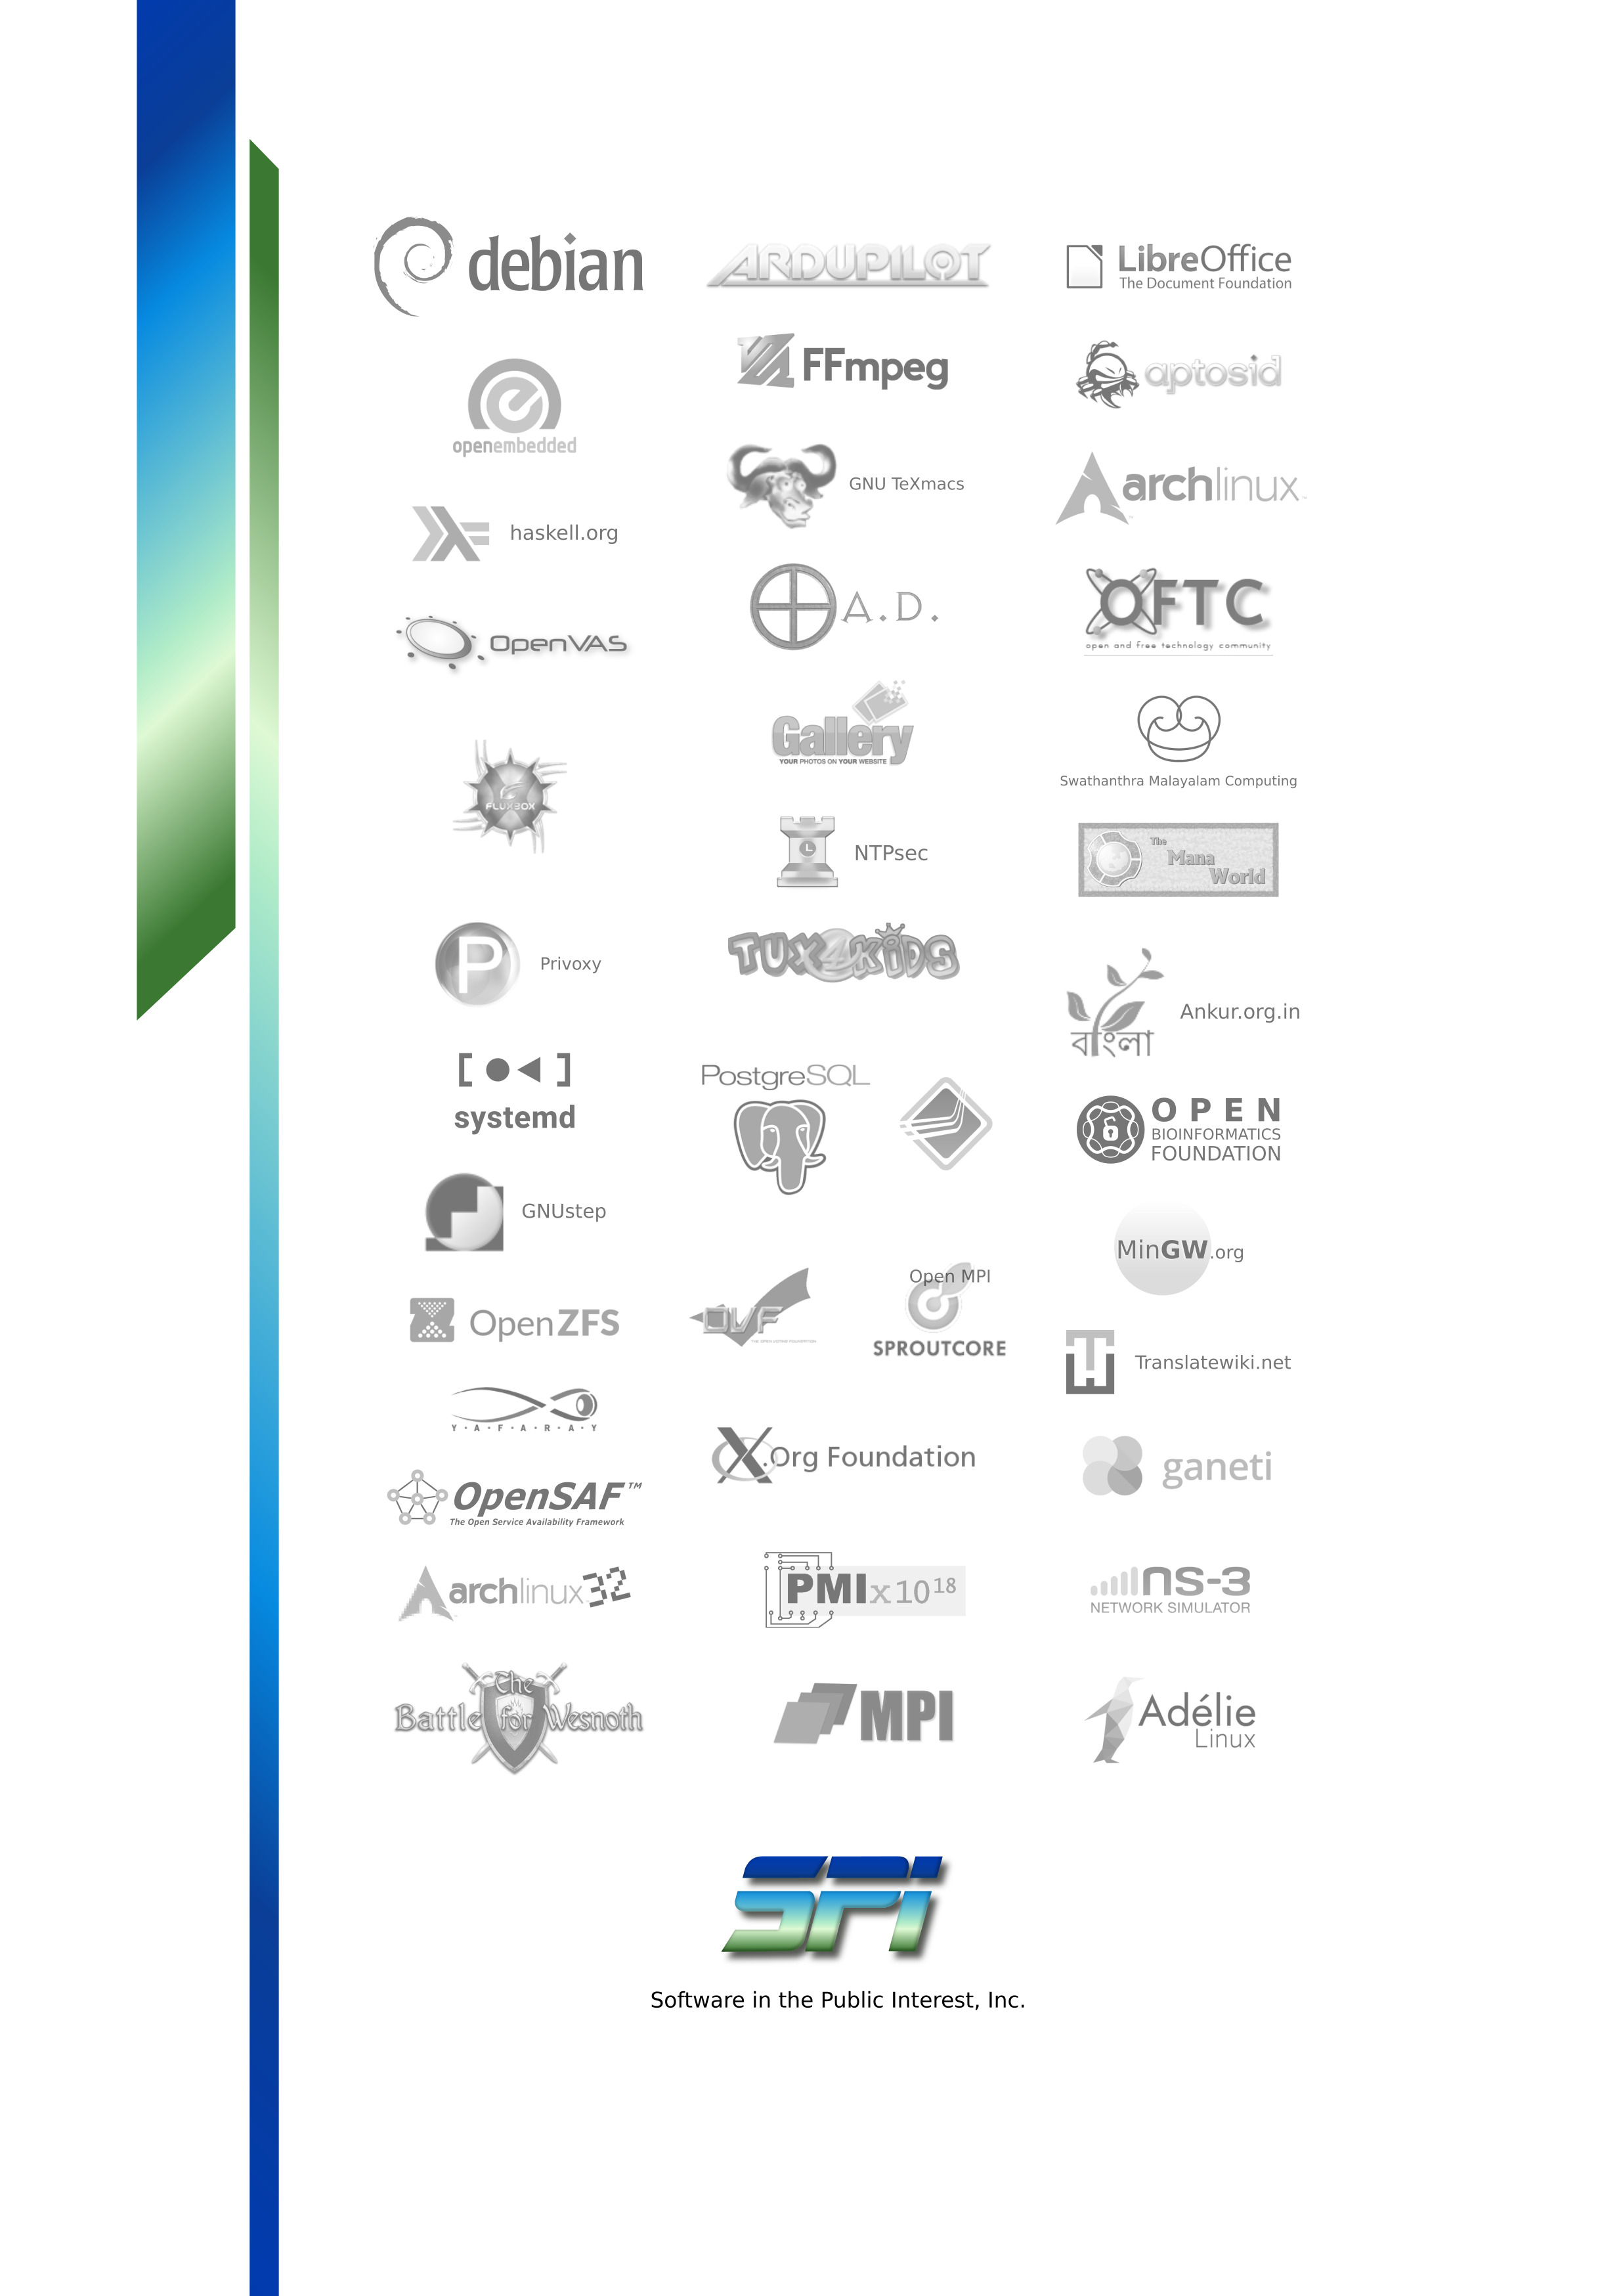
\includegraphics[width=\paperwidth,height=\paperheight]{images/spi-back-2022.jpg}}
}

\null

\end{document}
% Keep this at the bottom, thanks.
% Local Variables:
% TeX-master: "report"
% End:
